\documentclass{article}
\usepackage[catalan]{babel}
\usepackage[latin1]{inputenc}   % Permet usar tots els accents i car�ters llatins de forma directa.
\usepackage{enumerate}
\usepackage{amsfonts, amscd, amsmath, amssymb}
\usepackage[pdftex]{graphicx}
\usepackage{longtable}

\setlength{\textwidth}{16cm}
\setlength{\textheight}{24.5cm}
\setlength{\oddsidemargin}{-0.3cm}
\setlength{\evensidemargin}{0.25cm} \addtolength{\headheight}{\baselineskip}
\addtolength{\topmargin}{-3cm}

\newcommand\Z{\mathbb{Z}}
\newcommand\R{\mathbb{R}}
\newcommand\N{\mathbb{N}}
\newcommand\Q{\mathbb{Q}}
\newcommand\K{\Bbbk}
\newcommand\C{\mathbb{C}}

\newcounter{exctr}
\newenvironment{exemple}
{ \stepcounter{exctr} 
\hspace{0.2cm} 
\textit{Exemple  \arabic{exctr}: }
\it
\begin{quotation}
}{\end{quotation}}


\begin{document}

\textbf{\Large Tema 3.An\`alisi transformat (transformada Z)}

\vskip 0.2 cm

La transformada Z permet caracteritzar els sistemes digitals i estudiar, 
de manera relativament senzilla, algunes de les seves propietats (estabilitat, causalitat, etc.).

\vskip 0.3 cm
\noindent
\textbf{Transformada Z}

\vskip 0.2 cm
\noindent
Es defineix la transformada Z d'un senyal discret $x[n]$ com:
\[
X(z)={\cal Z} \{x[n]\})=\sum_{n=-\infty}^{+\infty} x[n] z^{-n}
\]

\noindent
on $z$ \'es una variable complexa. En funci\'o del valor de $z$ aquest sumatori pot 
\'esser infinit (s\`erie divergent). Anomenam \textbf{regi\'o de converg\`encia (ROC)}
el conjunt de valors de $z$ que fan que la s\`erie sigui convergent.

\vskip 0.5 cm
\noindent
Exemples:

\vskip 0.2 cm
\begin{tabular}{l|l|l}
$x[n]$ & $X(z)$ & ROC \\ \hline  & & \\
$\{\underline{1}, 2, 5, 7, 0, 1 \}$ & $1+2z^{-1}+5z^{-2}+7z^{-3}+z^{-5}$ &
pla $z$, excepte $z=0$ \\ \hline  & & \\
$\{1, 2, \underline{5}, 7, 0, 1 \}$ & $z^2+2z+5+7z^{-1}+z^{-3}$ &
pla $z$, excepte $z=0$ i $z=\infty$ \\ \hline  & & \\
$\delta[n]$ & $1$ & tot el pla $z$ \\ \hline  & & \\
$\delta[n-k]$ ($k > 0$) & $z^{-k}$ ($k > 0$) & pla $z$, excepte $z=0$ \\ \hline  & & \\
$\delta[n+k]$ ($k > 0$) & $z^{k}$ ($k > 0$) & pla $z$, excepte $z=\infty$ \\ \hline  & & \\
$(\frac{1}{2})^n u[n]$ & $\sum_{n=0}^{\infty} \left(\frac{1}{2} z^{-1} \right)^n=\displaystyle \frac{1}{1-\frac{1}{2}z^{-1}}$ &
$|z| > \frac{1}{2}$ \\ \hline  & & \\
$-(\frac{1}{2})^n u[-n-1]$ & $-\sum_{n=-\infty}^{1} \left( \frac{1}{2} z^{-1} \right)^n=\displaystyle \frac{1}{1-\frac{1}{2} z^{-1}}$ &
$|z| < \frac{1}{2}$ \\ \hline  & & \\
$2^n u[n] + 5^n u[-n-1]$ & 
$\sum_{n=0}^{\infty} \left(2 z^{-1} \right)^n + \sum_{n=-\infty}^{1} \left( 5 z^{-1} \right)^n=\frac{1}{1-2 z^{-1}} - \frac{1}{1-5 z^{-1}}$ &
$2 < |z| < 5$ \\ \hline 
\end{tabular}

\vskip 0.7 cm
\noindent
Observem que en els 5 primers exemples els senyals s\'on de duraci\'o finita mentre que els
4 darrers s\'on de duraci\'o infinita. En els primers casos la ROC \'es igual a tot el pla
excepte, possiblement, els punts $z=0$ i/o $z=\infty$.
En el cas dels senyals infinits la ROC, en general, t\'e la forma seg\"uent (forma d'anell):
$r_2 < |z| < r_1$, on $r_2$ i $r_1$ s\'on dos valors constants que depenen de la definici\'o de $x[n]$.

\vskip 0.5 cm
\noindent
Un senyal $x[n]$ queda totalment determinat per la seva transformada Z i la seva ROC. Con\`eixer
nom\'es la transformada Z no permet saber quin era el senyal original (veure exemples 6 i 7).

\vskip 0.5 cm
\noindent
Per als senyals causals ($x[n]=0$ si $n < 0$) la ROC t\'e la forma $|z| > r$, mentre per 
als no causals ($x[n]=0$ si $n \geq 0$) la ROC \'es de la forma $|z| < r$, per a alguna
constant $r$  (veure exemples 6 i 7).

\begin{figure}[htbp]
\begin{center}
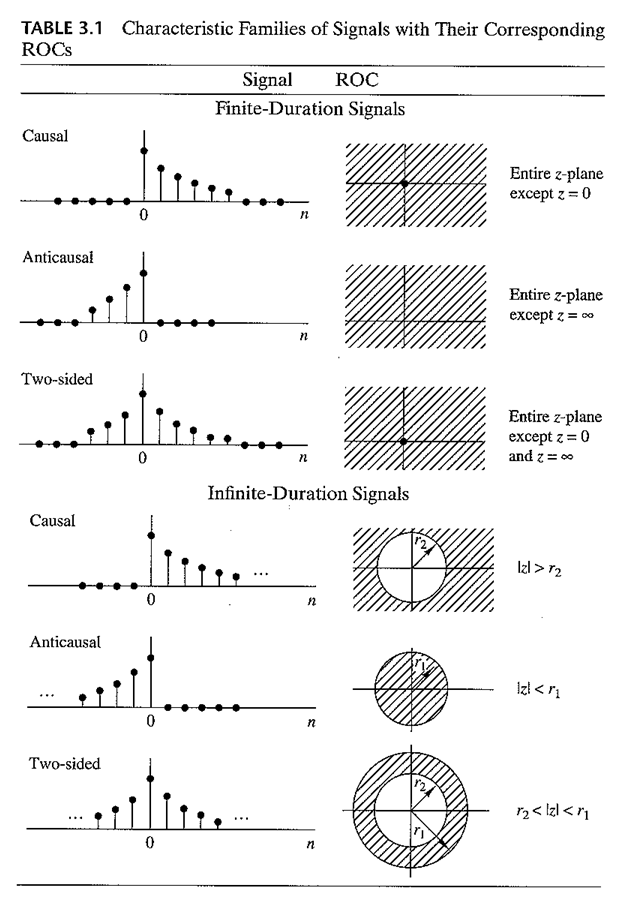
\includegraphics[width=12cm]{signalROC.png}
\end{center}
\caption{Font: Digital Signal Processing, J. Proakis, D. Manolakis, Pearson Prentice Hall, 2007}
\end{figure}

\newpage
%\vskip 0.3 cm
\noindent
\textbf{Propietats de la transformada Z}

\vskip 0.2 cm
\noindent
Denotam $X(z)={\cal Z} \{ x[n] \}$, amb ROC=$\text{ROC}_0 = r_2 < |z| < r_1$,
$X_1(z)={\cal Z} \{ x_1[n] \}$ amb ROC=$\text{ROC}_1$ i
$X_2(z)={\cal Z} \{ x_2[n] \}$ amb ROC=$\text{ROC}_2$.

\begin{enumerate}
\item Linealitat. 

\[
{\cal Z} \{ a_1 x_1[n] + a_2 x_2[n] \} = a_1 X_1(z) + a_2 X_2(z) 
\]

amb ROC=com a m\'inim, intersecci\'o de $\text{ROC}_1$ i $\text{ROC}_2$.

\item Despla\c{c}ament en temps.
\[
{\cal Z} \{ x[n-k] \} = z^{-k} X(z)
\]

amb ROC=$\text{ROC}_0$ excepte $z=0$ si $k > 0$ i $z=\infty$ si $k < 0$. 

\item Escalat.
\[
{\cal Z} \{ a^n x[n] \} = X(a^{-1} z) 
\]

amb ROC=$|a| r_2 < |z| < |a| r_1$.

\item Inversi\'o temporal.
\[
{\cal Z} \{ x[-n] \} = X(z^{-1}) 
\]

amb ROC=$\frac{1}{r_1} < |z| < \frac{1}{r_2}$.


\item Derivaci\'o en el domini $z$.
\[
{\cal Z} \{ nx[n] \} = -z \frac{d \, X(z) }{dz} 
\]

amb ROC=$\text{ROC}_0$.


\item Conjugaci\'o.
\[
{\cal Z} \{ x^*[n] \} = X^*(z^*) 
\]

amb ROC=$\text{ROC}_0$.

\item Convoluci\'o.
\[
{\cal Z} \{ x_1[n] * x_2[n] \} = X_1(z) X_2(z)
\]

amb ROC=com a m\'inim, intersecci\'o de $\text{ROC}_1$ i $\text{ROC}_2$.


\end{enumerate}

%\begin{figure}[htbp]
%\begin{center}
%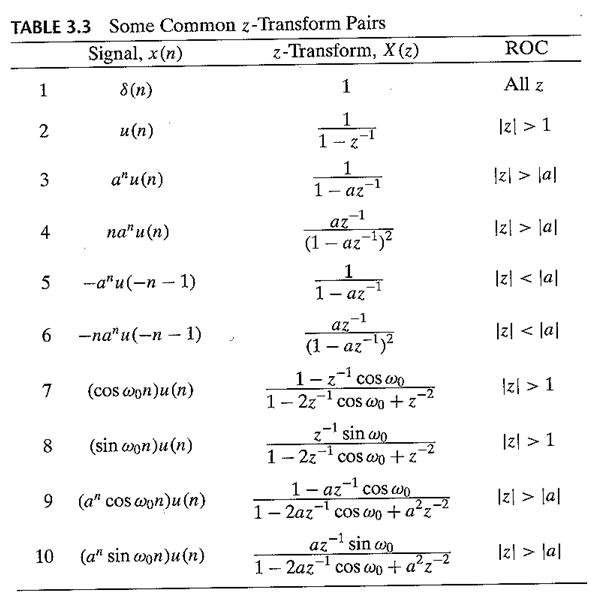
\includegraphics[width=12cm]{TZhabituals.png}
%\end{center}
%\caption{Font: Digital Signal Processing, J. Proakis, D. Manolakis, Pearson Prentice Hall, 2007}
%\end{figure}

\vskip 0.5cm
\noindent
\textbf{Transformades Z habituals}
\vskip 0.3 cm

\begin{tabular}{ccc}
\begin{tabular}{c|c|c}
$x[n]$ & $X(z)$ & ROC \\ \hline & &  \\
$\delta[n]$ & $1$ & tot $z$ \\ & & \\
$u[n]$ & $\frac{1}{1-z^{-1}}$ & $|z| > 1$ \\ & & \\
$a^nu[n]$ & $\frac{1}{1-az^{-1}}$ & $|z| > |a|$ \\ & & \\
$na^nu[n]$ & $\frac{az^{-1}}{(1-az^{-1})^2}$ & $|z| > |a|$ \\ & & \\
$-a^nu[-n-1]$ & $\frac{1}{1-az^{-1}}$ & $|z| < |a|$ 
\end{tabular}
&
$\qquad$
&
\begin{tabular}{c|c|c}
$x[n]$ & $X(z)$ & ROC \\ \hline & &  \\
$-na^nu[-n-1]$ & $\frac{az^{-1}}{(1-az^{-1})^2}$ & $|z| < |a|$ \\ & & \\
$\cos(\omega_0n) u[n]$ & $\frac{1-z^{-1}\cos \omega_0}{1-2z^{-1}\cos\omega_0+z^{-2}}$ & $|z|>1$ \\ & & \\
$\sin(\omega_0n) u[n]$ & $\frac{z^{-1}\sin \omega_0}{1-2z^{-1}\cos\omega_0+z^{-2}}$ & $|z|>1$ \\ & & \\
$(a^n\cos(\omega_0n)) u[n]$ & $\frac{1-az^{-1}\cos \omega_0}{1-2az^{-1}\cos\omega_0+a^2z^{-2}}$ & $|z|>|a|$ \\ & & \\
$(a^n\sin(\omega_0n)) u[n]$ & $\frac{az^{-1}\sin \omega_0}{1-2az^{-1}\cos\omega_0+a^2z^{-2}}$ & $|z|>|a|$ 
\end{tabular}
\end{tabular}


\newpage
\noindent
\textbf{Transformades Z racionals}

\vskip 0.3cm
\noindent
Un tipus important de transformades Z s\'on les transformada Z racionals,
que s'escriuen com a quocient de dos polinomis:

\begin{equation}
X(z)=\frac{P(z)}{Q(z)}=\frac{b_0+b_1z^{-1}+\cdots+b_Mz^{-M}}{a_0+a_1z^{-1}+\cdots+a_Nz^{-N}}=
\frac{b_0}{a_0} z^{N-M} \frac{(z-z_1)(z-z_2) \cdots (z-z_M)}{(z-p_1)(z-p_2) \cdots (z-p_N)}
\end{equation}

\vskip 0.3cm
\noindent
\textbf{Pols i zeros de la transformada Z}. S'anomenen \textbf{zeros} de $X(z)$ els valors de $z$ que fan
que $X(z)=0$. S'anomenen \textbf{pols} de $X(z)$ els valors de $z$ que fan que $X(z)=\infty$. 


\vskip 0.3cm
\noindent
Amb la factoritzaci\'o de l'equaci\'o anterior, $z_1, z_2, \cdots, z_M$ s\'on zeros de la transformada racional
i $p_1, p_2, \cdots, p_N$ s\'on pols. A m\'es, si $N > M$, $z=0$ \'es zero de $X(z)$ (amb multiplicitat $N-M$) 
i si $N < M$, $z=0$ \'es pol de $X(z)$ (amb multiplicitat $M-N$). Si els polinomis $P(z)$ i $Q(z)$ tenen arrels
en com\'u llavors haur\`a zeros i pols que es cancel.laran mutuament.

\vskip 0.3cm
\noindent
A $\infty$ existeix un zero si $X(\infty)=0$ i hi existeix un pol si $X(\infty)=\infty$. Si comptam els zeros
i pols a $\infty$, $X(z)$ t\'e el mateix nombre de pols i zeros.

\vskip 0.3cm
\noindent
Els pols i els zeros de $X(z)$ es representen en un \textbf{diagrama de zeros i pols}. La ROC de $X(z)$ no
cont\'e cap pol.

\vskip 0.3cm
\noindent
Exemples:

\begin{tabular}{l|c}
 & diagrama pols-zeros \\ \hline &  \\
 
\begin{tabular}{l}
$x[n]=a^n u[n] \qquad (a > 0)$ \\ \\
$X(z)=\frac{1}{1-az^{-1}}=\frac{z}{z-a}$ \\ \\
$\text{ROC:  } |z| > |a|$ \\ \\
$\text{zeros:  } z_1=0$ \\ \\
$\text{pols:  } p_1=a $
\end{tabular}


&

\begin{minipage}{5cm} 
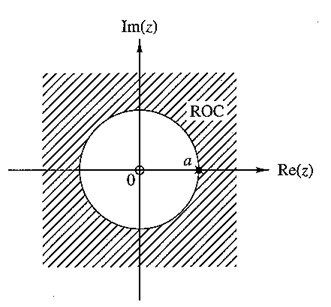
\includegraphics[width=5cm]{ex1PolsZeros.png}
\end{minipage} \\ \hline & \\

\begin{tabular}{l}
$x[n]=\begin{cases}a^n & \text{si } 0 \leq n \leq M-1 \\ $0$ & \text{altrament} \end{cases} \, (a>0, \text{real})$\\ \\ 
$X(z)=\frac{z^M-a^M}{z^{M-1}(z-a)}$ \\ \\
$\text{ROC:  } z \neq 0$ \\ \\
$\text{zeros:  } z_i=ae^{j 2\pi k/M}, \qquad i=1,\cdots, M-1$\\ \\
$\text{pols:  } p=0 \,\, \text{(multiplicitat $M-1$)}$
\end{tabular}


&

\begin{minipage}{5cm} 
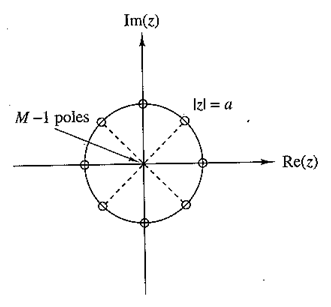
\includegraphics[width=5cm]{ex2PolsZeros.png}
\end{minipage} (M=8)

\end{tabular}


\newpage
\noindent
\textbf{Posici\'o dels pols i estabilitat de senyals causals reals}

\vskip 0.2 cm
\noindent
\textbf{Cas 1}. Senyal real amb un \'unic pol: $x[n]=a^nu[n]$, $X(z)=\frac{1}{1-az^{-1}}$, ROC=$|z|>|a|$, ($a$ real)
\begin{center}
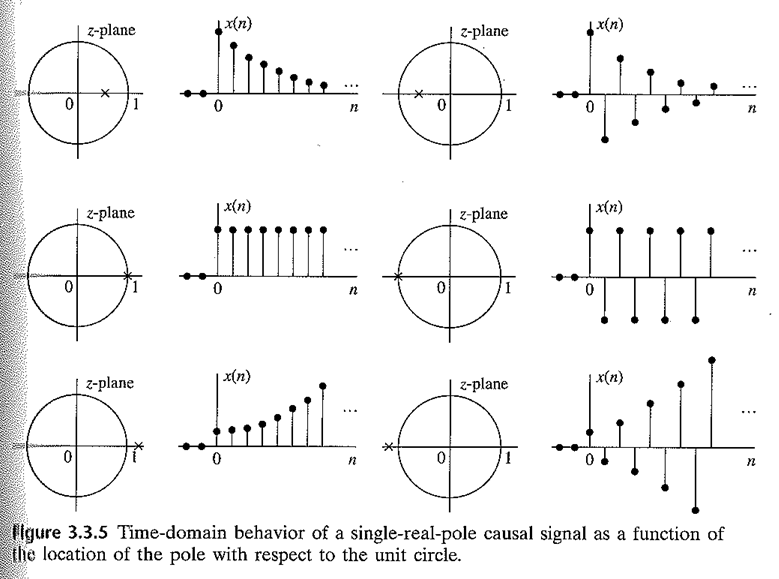
\includegraphics[width=12cm]{singlepole.png}
\end{center}

\vskip 0.2 cm
\noindent
\textbf{Cas 2}. Senyal real amb dos pols reals: $x[n]=n a^nu[n]$, $X(z)=\frac{az^{-1}}{(1-az^{-1})^2}$, ROC=$|z|>|a|$, ($a$ real)
\begin{center}
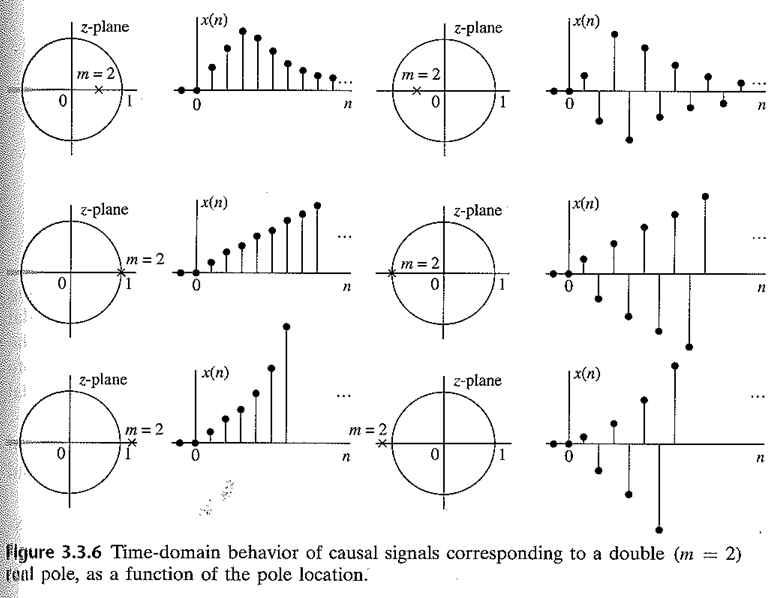
\includegraphics[width=12cm]{doublerealpole.png}
\end{center}

\newpage
\noindent
\textbf{Cas 3}. Senyal real amb un parell de pols complexes conjugats: $x[n]=(a^n \cos(\omega_0 n) ) u[n]$, 
$X(z)=\frac{1-az^{-1}\cos(\omega_0)}{1-2az^{-1}\cos(\omega_0)+a^2z^{-2}}$, ROC=$|z|>|a|$, ($a$ real)
\begin{center}
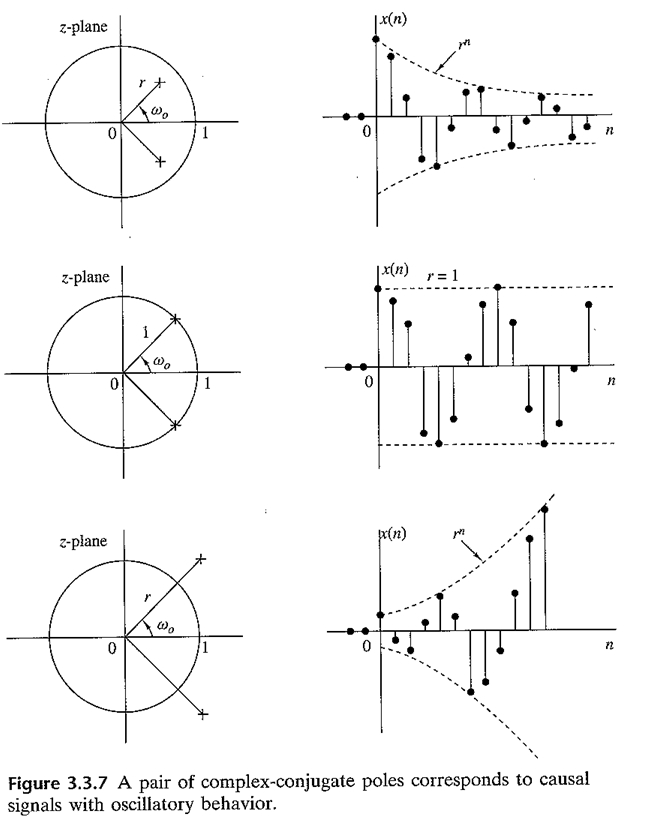
\includegraphics[width=12cm]{doublecomplexpole.png}
\end{center}

\vskip 0.5 cm
\noindent
En general podem afirmar que els senyals causals reals amb els pols a l'interior del \textbf{cercle unitat} ($|z|=1$)
s\'on fitats en amplitud. Si els pols estan a l'exterior del cercle unitat els senyals no s\'on fitats i
si els pols estan damunt el cercle unitat els senyals s\'on fitats si els pols tenen multiplicitat 1.
A m\'es, per al cas de pols dins el cercle unitat el decreixement del senyal \'es m\'es r\`apid com m\'es
a prop de l'origen es troben els pols.

\newpage
\noindent
\textbf{Inversi\'o de transformades Z racionals}

\vskip 0.2 cm
\noindent
L'objectiu \'es trobar $x[n]$ a partir de $X(z)=\frac{B(z)}{A(z)}=
\frac{b_0+b_1z^{-1}+\cdots+b_Mz^{-M}}{1+a_1z^{-1}+\cdots+a_Nz^{-N}}$ i la seva ROC.
El procediment \'es el seg\"uent:

\begin{enumerate}
\item si $M \geq N$ dividim els polinomis fins a trobar una expressi\'o amb la forma seg\"uent:
\[
X(z)=c_0+c_1z^{-1}+\cdots+c_{M-N} z^{-(M-N)}+\frac{B'(z)}{A(z)}
\]

on es compleix que $\frac{B'(z)}{A(z)}=\frac{b^{'}_0+b^{'}_1z^{-1}+\cdots+b^{'}_Kz^{-K}}{1+a_1z^{-1}+\cdots+a_Nz^{-N}}$
amb $K < N$.

El senyal $x_0[n]$ corresponent a $X_0(z)= c_0+c_1z^{-1}+\cdots+c_{M-N} z^{-(M-N)}$ \'es 
$x_0[n]=\{\underline{c_0}, c_1, \cdots, c_{M-N}\}$.

\item si $M < N$ (suposant $a_N \neq 0$):
\begin{enumerate}
\item descomposam la funci\'o racional en factors:
\begin{enumerate}
\item reescrivim $X(z)=\frac{B(z)}{A(z)}$ de la forma 
\[
\frac{X(z)}{z}=\frac{B'(z)}{A'(z)}=\frac{b^{'}_0 z^{N-1} + b^{'}_1 z^{N-2} + \cdots + b^{'}_N z^{N-M-1}}{z^N+a^{'}_1 z^{N-1} + \cdots + a^{'}_N}
\]
\item trobam les arrels de $A'(z)$
\item si totes les arrels s\'on diferents: 
\[
\frac{X(z)}{z}= \frac{A_1}{z-p_1} + \frac{A_2}{z-p_2} + \cdots + \frac{A_N}{z-p_N}
\]
\item si alguna arrel $p_i$ t\'e multiplicitat $k > 1$ la descomposici\'o en factors corresponent a
aquesta arrel \'es
\[
\frac{A_{1i}}{z-p_i} + \frac{A_{2i}}{(z-p_i)^2} + \cdots + \frac{A_{ki}}{(z-p_i)^k}
\]
\item trobam les constants $A_1, \cdots, A_N$ per igualaci\'o amb l'expressi\'o de $\frac{X(z)}{z}$
\end{enumerate}
\item escrivim $X(z)$ de la forma:
\[
X(z)= \frac{A_1}{1-p_1z^{-1}} + \frac{A_2}{1-p_2z^{-1}} + \cdots + \frac{A_{1i}}{1-p_i z^{-1}} + \frac{A_{2i} z^{-1}}{(1-p_i z^{-1})^2} + 
\cdots + \frac{A_N}{1-p_Nz^{-1}}
\]
\item calculam el senyal corresponent a cada sumand de $X(z)$, tenint en compte les seg\"uents propietats:
\[
\begin{array}{c|c|cr}
X(z) & \text{ROC} & x[n] & \\ \hline & & & \\
\frac{1}{1-pz^{-1}} & |z|>|p| & p^n u[n] & \text{(senyal causal)} \\ & & & \\
\frac{1}{1-pz^{-1}} & |z|<|p| & -p^n u[-n-1] & \text{(senyal anticausal)} \\ & & & \\
\frac{A}{1-pz^{-1}}  + \frac{A^*}{1-p^*z^{-1}} & |z|>|p| & 2 |A| r^n \cos(\beta n + \alpha) u[n] & 
A=|A|e^{j\alpha}, \,\, r=|r|e^{j\beta}, \,\, \text{(senyal causal)} \\ & & & \\
\frac{pz^{-1}}{(1-pz^{-1})^2} & |z|>|p| & np^nu[n] & \text{(senyal causal)}
\end{array}
\]

\end{enumerate}

\end{enumerate}


\vskip 0.5 cm
\noindent
\textbf{Exemple}: determinau el sistema causal que t\'e per transformada 
\[
X(z)=\frac{1}{(1+z^{-1})(1-z^{-1})^2}
\]

\vskip 0.3 cm
\noindent
\textbf{Soluci\'o}:
\begin{enumerate}
\item en aquest cas $M=0$ i $N=3$, per tant $M < N$. Reescrivim la transformada de
la forma:
\[
X(z)=\frac{z^3}{(z+1)(z-1)^2} \qquad \Longrightarrow \qquad \frac{X(z)}{z}=\frac{z^2}{(z+1)(z-1)^2}
\]
\item les arrels de $(z+1)(z-1)^2$ s\'on $p_1=-1$ i $p_2=1$ (doble), per tant podem descomposar $X(z)/z$
de la seg\"uent manera:
\[
\frac{X(z)}{z}=\frac{z^2}{(z+1)(z-1)^2}=\frac{A_1}{z+1}+\frac{A_2}{z-1}+\frac{A_3}{(z-1)^2}
\]
\item calculam les constants per comparaci\'o dels numeradors de les expressions anteriors i trobam 
$A_1=\frac{1}{4}$, $A_2=\frac{3}{4}$ i $A_3=\frac{1}{2}$. Per tant:
\[
X(z)=\frac{1}{4} \frac{1}{1+z^{-1}} + \frac{3}{4} \frac{1}{1-z^{-1}} + \frac{1}{2} \frac{z^{-1}}{(1-z^{-1})^2} 
\]
\item mirant les taules de transformades Z habituals trobam les transformades de cada sumand, tenint
en compte que el senyal que buscam \'es causal:
\[
x[n]=\frac{1}{4} (-1)^nu[n] + \frac{3}{4} u[n] + \frac{1}{2} n (1)^n u[n] = 
\left( \frac{1}{4} (-1)^n + \frac{3}{4} + \frac{1}{2} n \right) u[n]
\]
\end{enumerate}

\vskip 1cm
\noindent
\textbf{Inversi\'o de transformades Z descrites com a s\`eries de pot\`encies}

\vskip 0.2 cm
\noindent
Si una $X(z)$ amb una determinada ROC es pot escriure de la seg\"ent manera:
\[
X(z)=\sum_{n=-\infty}^{\infty} c_n z^{-n}
\]
\noindent
i aquesta s\`erie convergeix dins la ROC donada, llavors $x[n]=c_n$, per a tot $n$.

\vskip 0.2 cm
\noindent
Exemples:
\vskip 0.2 cm
\begin{tabular}{l|l|l}
$X(z)$ & ROC & $x[n]$ \\ \hline & & \\
$\frac{1}{1-1.5z^{-1}+0.5z^{-2}}$ & $|z|>1$ & $\{\underline{1}, \frac{3}{2}, \frac{7}{4}, \cdots \}$ \\ \hline & & \\
$\frac{1}{1-1.5z^{-1}+0.5z^{-2}}$ & $|z|<0.5$ & $\{ \cdots, 14, 6, 2, 0, \underline{0} \}$ \\ \hline & & \\
$\log(1+az^{-1})$ & $|z|>|a|$ & $\begin{cases} (-1)^{n+1} \frac{a^n}{n} & \text{si }n \geq 1 \\ \\ 0 & \text{si } n \leq 0 \end{cases}$
\\ & & (Nota: $\log(1+x)=\sum_{n=1}^\infty \frac{ (-1)^{n+1} x^n}{n}$ si $|x|<1$)
\end{tabular}


\newpage
\noindent
\textbf{An\`alisi de sistemes LTI mitjan\c{c}ant la transformada Z}

\vskip 0.3 cm
\noindent
Recordem que la resposta d'un sistema LTI a una entrada $x[n]$ es pot escriure com
\[
y[n]=h[n] * x[n]
\]
\noindent
on $h[n]$ \'es la resposta impulsional del sistema.

\vskip 0.2 cm
\noindent
Aplicant les propietats de la transformada Z podem escriure l'expressi\'o anterior
de la seg\"uent manera:
\[
Y(z)=H(z) X(z)
\]
\noindent
on $X(z)$, $Y(z)$ i $H(z)$ s\'on les transformades Z de $x[n]$, $y[n]$ i $h[n]$, respectivament.
$H(z)$ rep el nom de \textbf{funci\'o de transfer\`encia} del sistema.

\vskip 0.2 cm
\noindent
Si coneixem l'entrada i la sortida del sistema podem calcular $H(z)$:
\[
H(z)=\frac{Y(z)}{X(z)}
\]

\vskip 0.2 cm
\noindent
Si la relaci\'o entre $x[n]$ i $y[n]$ s'expressa mitjan\c{c}ant una equaci\'o en difer\`encies
finites podem calcular $H(z)$ amb la f\`ormula anterior i utilitzant les propietats de la transformada Z.

\vskip 0.2 cm
\noindent
\textbf{Exemple}: determinau la resposta impulsional del sistema causal descrit per la seg\"uent equaci\'o
\[
y[n]=\frac{1}{2}y[n-1]+2x[n]
\]

\vskip 0.2 cm
\noindent
\textbf{Soluci\'o}: 
\begin{enumerate}
\item aplicam la transformada Z als dos membres de l'equaci\'o i aplicam propietats:
\[
Y(z)=\frac{1}{2}z^{-1}Y(z)+2X(z)
\]
\item escrivim la relaci\'o $Y(z)/X(z)$:
\[
Y(z)-\frac{1}{2}z^{-1}Y(z)=2X(z) \qquad \Longrightarrow \qquad H(z)=\frac{Y(z)}{X(z)}=\frac{2}{1-\frac{1}{2}z^{-1}}
\]
\item comparant amb la taula de transformades Z habituals trobam que 
\[
h[n]=2(\frac{1}{2})^n u[n]
\]
\noindent
ja que el sistema \'es causal i per tant $h[n]$ tamb\'e ho \'es.
\end{enumerate}


\vskip 0.5 cm
\noindent
\textbf{Causalitat i estabilitat de sistemes LTI}

\vskip 0.2 cm
\noindent
L'an\`alisi de $H(z)$ permet determinar de manera molt senzilla les caracter\'istiques de
causalitat i estabilitat d'un sistema LTI:
\begin{itemize}
\item Un sistema LTI \'es causal si i nom\'es si la ROC de $H(z)$ \'es l'exterior d'un cercle de
radi $r < \infty$, incloent el punt $z=\infty$.
\item Un sistema LTI \'es estable si i nom\'es si la ROC de $H(z)$ cont\'e el cercle unitat.
\item Un sistema LTI causal \'es estable si i nom\'es si tots els pols de $H(z)$ estan a l'interior 
del cercle unitat. 
\item Un sistema LTI causal amb pols al cercle unitat pot produir una sortida estable 
si el senyal d'entrada i H(z) no tenen pols en com\'u. 
\item La cancel.laci\'o de pols i zeros en l'expressi\'o de $H(z)$ pot produir sistemes 
estables que en la pr\`actica no ho s\'on degut a la imperfecta cancel.laci\'o dels pols i els zeros.
\end{itemize}
 

\end{document}

